\documentclass[letterpaper,11pt,twoside,]{pinp}

%% Some pieces required from the pandoc template
\providecommand{\tightlist}{%
  \setlength{\itemsep}{0pt}\setlength{\parskip}{0pt}}

% Use the lineno option to display guide line numbers if required.
% Note that the use of elements such as single-column equations
% may affect the guide line number alignment.

\usepackage[T1]{fontenc}
\usepackage[utf8]{inputenc}

% pinp change: the geometry package layout settings need to be set here, not in pinp.cls
\geometry{layoutsize={0.95588\paperwidth,0.98864\paperheight},%
  layouthoffset=0.02206\paperwidth, layoutvoffset=0.00568\paperheight}

\definecolor{pinpblue}{HTML}{185FAF}  % imagecolorpicker on blue for new R logo
\definecolor{pnasbluetext}{RGB}{101,0,0} %


\usepackage{booktabs}
\usepackage{longtable}
\usepackage{array}
\usepackage{multirow}
\usepackage{wrapfig}
\usepackage{float}
\usepackage{colortbl}
\usepackage{pdflscape}
\usepackage{tabu}
\usepackage{threeparttable}
\usepackage{threeparttablex}
\usepackage[normalem]{ulem}
\usepackage{makecell}

\title{Lab 007 - Inference for proportions.}

\author[a]{EPIB607 - Inferential Statistics}

  \affil[a]{McGill University}

\setcounter{secnumdepth}{5}

% Please give the surname of the lead author for the running footer
\leadauthor{Bhatnagar}

% Keywords are not mandatory, but authors are strongly encouraged to provide them. If provided, please include two to five keywords, separated by the pipe symbol, e.g:
 \keywords{  Sampling distribution |  Standard error |  Normal
distribution |  Quantiles |  Percentiles |  Z-scores  }  

\begin{abstract}

\end{abstract}

\dates{This version was compiled on \today} 

% initially we use doi so keep for backwards compatibility
% new name is doi_footer


\begin{document}

% Optional adjustment to line up main text (after abstract) of first page with line numbers, when using both lineno and twocolumn options.
% You should only change this length when you've finalised the article contents.
\verticaladjustment{-2pt}

\maketitle
\thispagestyle{firststyle}
\ifthenelse{\boolean{shortarticle}}{\ifthenelse{\boolean{singlecolumn}}{\abscontentformatted}{\abscontent}}{}

% If your first paragraph (i.e. with the \dropcap) contains a list environment (quote, quotation, theorem, definition, enumerate, itemize...), the line after the list may have some extra indentation. If this is the case, add \parshape=0 to the end of the list environment.


\begin{figure}[H]
  \begin{center}
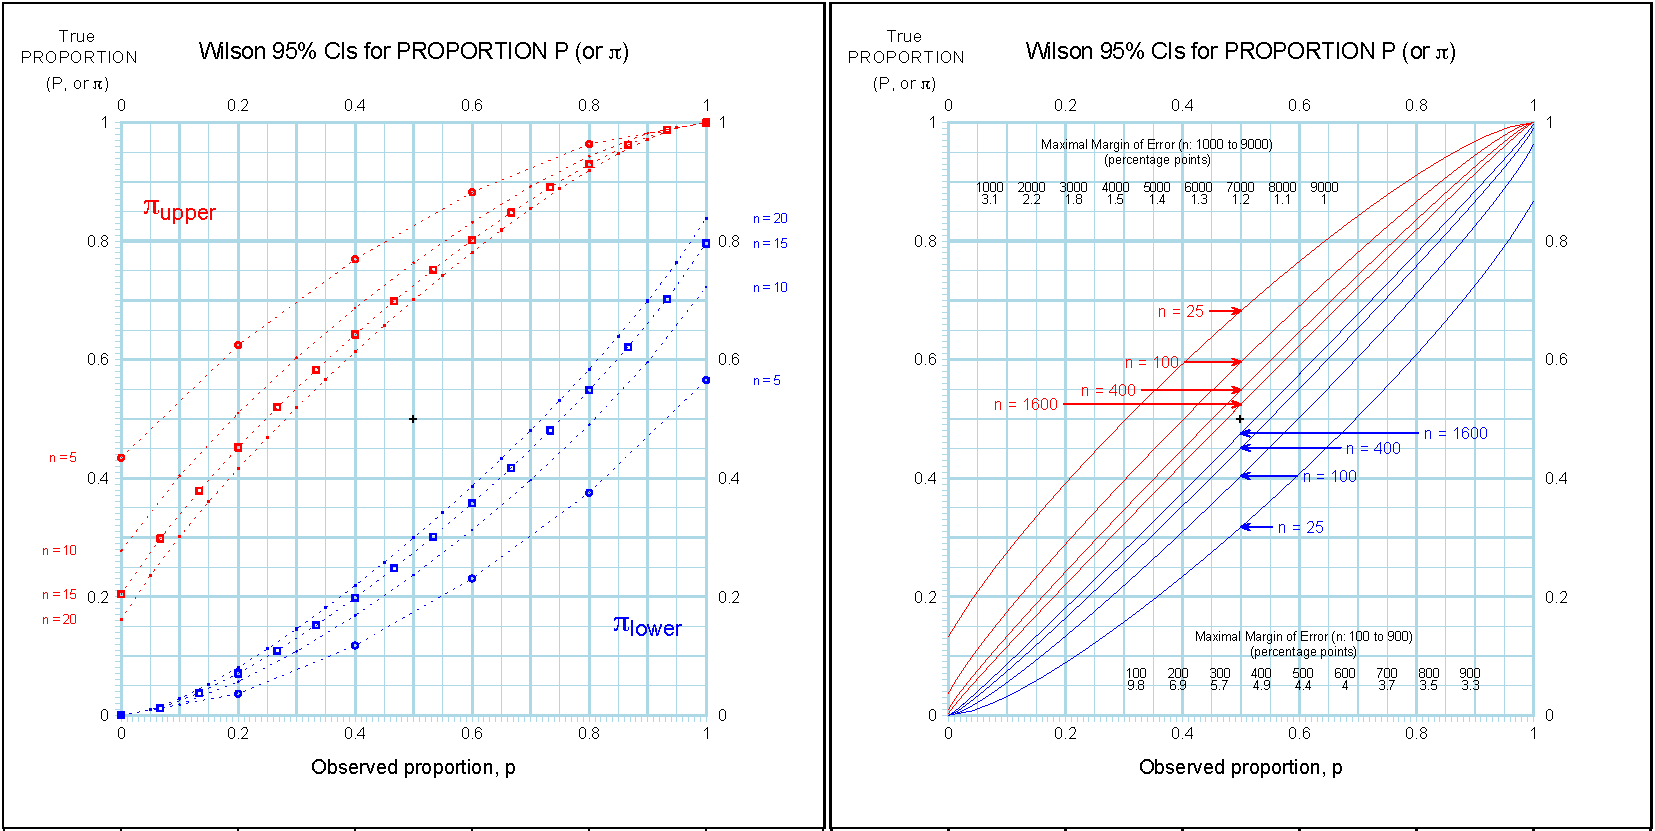
\includegraphics[scale=0.65]{Nomogram.pdf}
  \end{center}
  \caption{\normalsize Wilson 95\% CIs for proportion $\pi$}\label{fig:nomo}
\end{figure}

\hypertarget{drunken-cyclists}{%
\section{Drunken cyclists}\label{drunken-cyclists}}

In the United States approximately 900 people die in bicycle accidents
each year. One study examined the records of 1711 bicyclists aged 15 or
older who were fatally injured in bicycle accidents between 1987 and
1991 and were tested for alcohol. Of these, 542 tested positive for
alcohol (blood alcohol concentration of 0.01\% or higher).

\begin{enumerate}
\def\labelenumi{\alph{enumi}.}
\tightlist
\item
  To do statistical inference for these data, we think in terms of a
  model where \(p\) is parameter that represents the probability that a
  tested bicycle rider is positive for alcohol. Find a 99\% confidence
  interval for \(p\).
\item
  Can you conclude from your analysis of this study that alcohol causes
  fatal bicycle accidents? Explain
\item
  In this study 386 bicyclists had blood alcohol levels above 0.10\%, a
  level defining legally drunk in many states at the time. Give a 99\%
  confidence interval for the proportion who were legally drunk
  according to this criterion.
\end{enumerate}

\hypertarget{handling-contact-lenses}{%
\section{Handling contact lenses}\label{handling-contact-lenses}}

Failure to follow recommended contact lens wear and care practices can
lead to serious eye infection. A survey of a random sample of 281
Americans who wear contact lenses regularly asked about contact lens
practices. The survey found that 139 respondents do not consistently
wash their hands before handing their contact lenses.

\begin{enumerate}
\def\labelenumi{\alph{enumi}.}
\tightlist
\item
  Obtain a plus four 99\% confidence interval for the proportion \(p\)
  of all American contact lens wearers who do not consistently wash
  their hands before handing their lenses. Verify that the conditions
  for your confidence interval are met.
\item
  Obtain a large sample 99\% confidence interval for the proportion
  \(p\) of all American contact lens wearers who do not consistently
  wash their hands before handing their lenses. How does this compare to
  the interval you calculated in part (a)?
\item
  The researchers indicated that this survey had a substantial
  nonresponse rate. How does this information affect your interpretation
  of the confidence interval in context?
\item
  Survey participants simply answered a questionnaire, and no attempt
  was made to verify the answers. How does this information affect your
  interpretation of the confidence interval in context?
\end{enumerate}

\hypertarget{cancer-detecting-dogs}{%
\section{Cancer-detecting dogs}\label{cancer-detecting-dogs}}

A study was designed to determine whether dogs can be trained to
identify urine specimens from individuals with bladder cancer. Dogs were
first trained to discriminate between urine specimens from patients with
bladder cancer and urine specimens from patients with other conditions.
After the training was completed, the dogs had to pick one of seven new
urine specimens. Each time, only one of the seven urine specimens came
from a patient with bladder cancer. Out of 54 trials, the dogs
identified the correct urine specimen 22 times.

\begin{enumerate}
\def\labelenumi{\alph{enumi}.}
\tightlist
\item
  If the dogs were simply picking a urine specimen at random, we would
  expect them to be correct, on average, 1 out of 7 times. The
  experiment was designed to test whether dogs can perform better than
  chance. State the null and alternative hypotheses for this test.
\item
  Obtain the test statistic and the P-value. What do you conclude?
\end{enumerate}

\hypertarget{fall-2018-midterm-the-us-presidential-campaign-is-a-very-costly-affair.-one-punditcomedian-has-suggested-that-much-time-and-trouble-could-be-saved-if-the-candidates-simply-had-their-height-measured.-in-20-of-the-25-elections-where-the-data-are-known-the-taller-candidate-has-won.-tall-people-are-credited-with-qualities-expected-of-capable-people}{%
\section{(FALL 2018 Midterm) The US presidential campaign is a very
costly affair. One pundit/comedian has suggested that much time and
trouble could be saved, if the candidates simply had their height
measured. In 20 of the 25 elections where the data are known, the taller
candidate has won. Tall people are credited with qualities expected of
capable
people}\label{fall-2018-midterm-the-us-presidential-campaign-is-a-very-costly-affair.-one-punditcomedian-has-suggested-that-much-time-and-trouble-could-be-saved-if-the-candidates-simply-had-their-height-measured.-in-20-of-the-25-elections-where-the-data-are-known-the-taller-candidate-has-won.-tall-people-are-credited-with-qualities-expected-of-capable-people}}

\begin{enumerate}
\def\labelenumi{\alph{enumi}.}
\tightlist
\item
  In order to test this claim about tall people, we need to test it
  against a null hypothesis. State the null hypothesis in plain English.
\item
  Translate the null and the alternative hypotheses into statistical
  notation.
\item
  Write down the steps, including the \texttt{R} code, to carry out the
  statistical test. Include a sentence on how you would report your
  findings.
\item
  You don't have access to software to run the code you have suggested
  in part (c), but can you anticipate what your findings will be?
  Explain.
\end{enumerate}

%\showmatmethods


\bibliography{pinp}
\bibliographystyle{jss}



\end{document}
